% • Name the different pipeline steps.
% • Elaborate their purpose and implementation, including the used tools.
% • Discuss the data flow throughout the steps and name the relevant artifacts/data.
% A new team member should be able to understand your release processes and where the artifacts get published.

% Insufficient -> At least one of the pipelines is not documented.
% Sufficient -> Two pipeline for release a package and an image are described. All pipeline steps get introduced.
% Good -> The report describes the purpose of all pipeline steps and introduces the relevant tools. The documentation visualizes the pipelines and connects the text.
% Very Good -> The documentation introduces relevant artifacts/data and their dependencies/flow.
% Excellent -> The documentation makes it easy for new team members to get started with contributing to the project. It becomes easy to understand the build pipelines, e.g., how models and releases are built and where artifacts get published.
\section{Release Pipelines}
Because we adopt the micro-services architecture, instead of releasing the entire application in one single package, each individual component is released separately. This process of releasing varies depending on the type of component. Therefore, in order to automate these configurations we make use of {\color{blue} \href{https://docs.github.com/en/actions/using-workflows}{GitHub Actions}}, i.e. workflows.

\subsection{Software Package}
The first type of workflow is configured for a software package. During this process a repository is built, after which the artifact is stored in a package repository. For example, the workflow for \texttt{lib-version} publishes the library to {\color{blue} \href{https://github.com/features/packages}{GitHub Packages}}. Fig. {\color{red} \ref{fig:libversion-workflow}} shows a visualization of this process.

\subsubsection{Automatic Versioning}
Before releasing the package it is important that we update its version. For this we define another {\color{blue}\href{https://github.com/remla24-team12/lib-version/blob/main/.github/workflows/version.yml}{workflow}}, which is triggered by pushes directly to the main branch (which is a bad practice, but its included to be safe) or by pull requests to the main branch. The version itself is defined using a Git tag. The stages of this workflows are as follows:
\begin{itemize}
    \item \textbf{Increment version}: This stage looks up the latest tag and bumps it up. Currently, we always increment the patch for simplicity, meaning minor and major releases are not supported. This is a future improvement.
    \item \textbf{Create Git tag}: Once the new tag number has been computed, a new tag is created and pushed. 
\end{itemize}

The {\color{blue}\href{https://github.com/remla24-team12/lib-version/blob/main/.github/workflows/release.yml}{release workflow}} is triggered after the automatic versioning workflow has been completed.
Afterwards the following stages are executed:
\begin{itemize}
    \item \textbf{Get latest tag}: Retrieve the tag created in the versioning workflow.
    \item \textbf{Set up Node.js}: Configure Node.js environment to use GitHub Packages as the registry and set the appropriate scope.
    \item \textbf{Install dependencies}: Install necessary node packages as defined in package.json.
    \item \textbf{Update version}: Update the package.json file with the version from the latest git tag.
    \item \textbf{Build and publish package}: Builds the npm package and publishes it to GitHub Packages using the authentication token provided through a secret.
\end{itemize}

\begin{figure*}
    \centering
    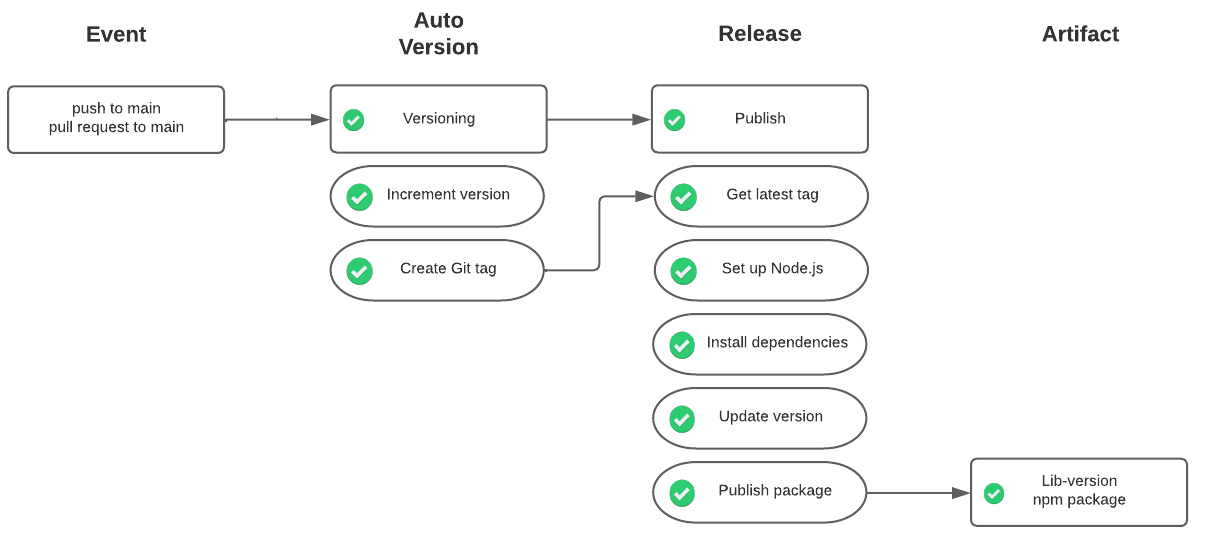
\includegraphics[width=0.75\linewidth]{images/libversion_workflow.png}
    \caption{Visualization of \texttt{lib-version} workflows}
    \label{fig:libversion-workflow}
\end{figure*}
% Visualization tool: 
% https://lucid.app/lucidchart/38c9ce70-2d27-459d-b58a-c52e3883af58/edit?beaconFlowId=119EFCC8C64C2A8A&invitationId=inv_871bb54d-8a09-4c35-afbd-f00ea69222e8&page=0_0#

\subsection{Container Image}
